\section{Aditya Dhoke (ME20B014)}
\vspace{0.25cm}
   % This document is about the Newton's Law of Gravitation.
\subsection{What is Newton's Law of Gravitation?}  
Newton's law of universal gravitation is usually stated as, " Every particle attracts every other particle in the universe with a force that is directly proportional to the product of their masses and inversely proportional to the square of the distance between their centers".
   The mathematical equation that gives the magnitude of the gravitational force between two point objects of mass  $ m_1 $ and $ m_2 $ at a distance 'r' from each other is:
   \begin{equation} \label{eq:1}
         F = \frac{Gm_1m_2}{r^2}
   \end{equation}
   Here , 'G' is the Universal Gravitational Constant 
          'F' is the Gravitational force experienced by the two point objects \par
          \begin{figure}[h]
          \begin{center}
          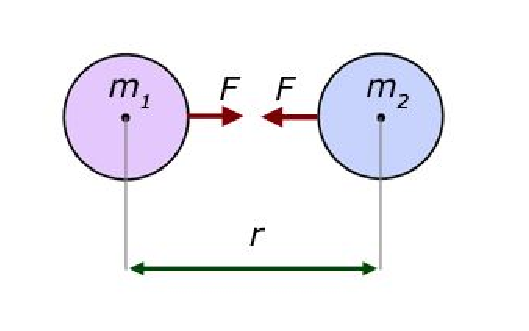
\includegraphics[scale=1]{me20b014/me20b014.eps} 
          \end{center}
          \caption{Newton's Law of Universal Gravitation}
          \label{fig1}
          \end{figure}
The Newton's Universal Gravitational Law can be beter understood through figure \ref{fig1}... \par
 Let's study each of the term in mathematical equation \ref{eq:1} of Newton's Law of Gravitation.
\subsection{Universal Gravitation Constant}
The Universal Gravitational Constant is denoted by the letter 'G'. It is the proportionality constant in the Newtons Law \ref{eq:1} that relates gravitational force between the two bodies to the product of their masses and the inverse of the square of the distance between them. The measured value of the constant in SI Units is $ 6.674x10^-11 m^3 kg^{-1} s^{-2} $ \par
\textbf{\bfseries \large Interesting Fact!} \par
The first direct measurement of gravitational attraction between two bodies in the laboratory was performed in 1798, seventy-one years after Newton's death, by Henry Cavendish. He determined a value for G implicitly, using a torsion balance invented by the geologist Rev. John Michell (1753).
\subsection{Mass of the Body}
 Mass is a property of physical body . It is also defined as a measure of its restistance to acceleration when a net force is 
applied. An object's mass also determines the strength of its gravitational attraction to other bodies.The SI Unit of mass is kilogram (kg). 
Sometimes people confuse mass with weight , however these are two different terms . Weight is a force which might be different for different magnitudes of gravtitaional force on the body whereas mass is constant for a physical body.
\subsection{Distance between two bodies}
In equation \ref{eq:1} , 'r' denotes the distance between the two bodies . It measures how much far away the two bodies are from each other.
We always consider perpendicular distance between the two bodies as shown in figure \ref{fig1}.The SI Unit of distnace is 'm' metre.
However, for planetary bodies , the distance is very huge and cannot be expressed shortly , so we use other units such as 'km' kilometre. 
\subsection{Force}
Force can be defined as any influence that can affect the motion of an object if un-opposed. Newton's Second Law defines force quantitatively as timed rate of change of momentum.The SI Unit of force is Newton. Sir Isaac Newton described the motion of all objects using the concepts of inertia and force, and in doing so he found they obey certain conservation laws which we today know as the "Newton's Laws of Motion". \par
Force is broadly divided into following categories : 
\begin{enumerate}
       \item Fundamental Forces
             \begin{itemize}
                    \item Gravitaional Force
                    \item Electromagnetic Force
                    \item Weak Nuclear Forces
                    \item Strong Nuclear Forces
             \end{itemize}
                    \item Non Fundamental Forces
                          \begin{itemize}
                                 \item Normal Force
                                 \item Friction Force
                                 \item Tension Force
                                 \item Elastic Force
                                 \item Fictitious Force
                          \end{itemize}
\end{enumerate}
The force in equation \ref{eq:1} is Gravtitaional Force. So , the force  which  attracts every particle to every other particle is called the gravitational force.This is a very long range force which exists even between planetry bodies. \par
\textbf{\bfseries \large Interesting Fact!} \par
The Gravitaional Force is responsible for the motion of planets around sun and the motion of moons around their respective planets! 
\subsection{Importance of Newton's Law of Universal Gravitation} 
Newton's Law of Universal gravitation is one of the most important and fundamental laws in classical physics . This is because it can be applied to almost every particle in the universe. It guides the 
efforts of scientists in their study of planetary orbits. Knowing that all objects exert gravitational influences on each other, the small 
deviations in a planet's elliptical motion can be easily explained. As the planet Jupiter approaches the planet Saturn in its orbit, it tends to 
deviate from its smooth path. This deviation is easily explained when considering the effect of the gravitational pul between Saturn and Jupiter.
Newton's comparison of the acceleration of the apple to that of the moon led to a surprisingly simple conclusion abou the nature of gravity that is woven into the entire universe. \par
    The equation \ref{eq:1} has been taken from the citation~\cite{Verlinde2011}
%\bibliography{Newton}
%\bibliographystyle{plain}              
